%% PH 5110 term paper -- one-column IEEE journal format (IEEEtran V1.8b, as in the course template)
\documentclass[journal,11pt]{IEEEtran}
\usepackage[T1]{fontenc}
\usepackage{amsmath,amssymb,bm}
\usepackage{graphicx}
\usepackage{booktabs}
\usepackage{url}
\usepackage{wrapfig}
\graphicspath{{figures/}{photos/}}

% ---- Peer editor(s): write the name(s) between the braces, e.g. \def\peereditors{A. Name and B. Name}
\def\peereditors{}

\usepackage{needspace}
\usepackage{ragged2e}
\usepackage{float}
\usepackage{dblfloatfix}
\setcounter{dbltopnumber}{2}\renewcommand{\dbltopfraction}{0.92}\renewcommand{\topfraction}{0.9}\renewcommand{\textfraction}{0.08}\renewcommand{\floatpagefraction}{0.85}\renewcommand{\dblfloatpagefraction}{0.85}
\newcommand{\shead}[1]{\par\vspace{5pt}\noindent\textbf{#1:}\par\nopagebreak\vspace{2pt}\noindent\ignorespaces}
\newcommand{\mhead}[1]{\par\vspace{3pt}\noindent\emph{#1:}\par\nopagebreak\vspace{1pt}\noindent\ignorespaces}
\newcommand{\ka}{\kappa_1}
\newcommand{\kc}{\kappa_2}
\newcommand{\kb}{\bar\kappa}
\newcommand{\dd}{\mathrm{d}}
\newcommand{\Tr}{\mathrm{Tr}}
\setlength{\textfloatsep}{6pt plus 2pt minus 2pt}\setlength{\dbltextfloatsep}{8pt plus 2pt minus 2pt}
\setlength{\floatsep}{6pt plus 2pt minus 2pt}
\setlength{\abovecaptionskip}{3pt}

\usepackage{environ}
\usepackage{adjustbox}
\newcommand{\dmath}[1]{\[\adjustbox{max width=0.95\columnwidth}{$\displaystyle #1$}\]}
\makeatletter
\let\topq@origlabel\label
\RenewEnviron{equation}{\refstepcounter{equation}\protected@edef\topq@lbl{\@currentlabel}%
\[\let\label\topq@origlabel\adjustbox{max width=0.85\columnwidth}{$\displaystyle\BODY$}\quad(\theequation)\]\ignorespacesafterend}
\makeatother
\raggedbottom
\linespread{0.97}\begin{document}
\hyphenpenalty=10000 \exhyphenpenalty=10000 \emergencystretch=2em \clubpenalty=1000 \widowpenalty=1000 \displaywidowpenalty=50 \predisplaypenalty=200 \interlinepenalty=0
\abovedisplayskip=5pt plus 1pt minus 1pt \belowdisplayskip=5pt plus 1pt minus 1pt
\abovedisplayshortskip=3pt \belowdisplayshortskip=4pt

\title{\LARGE TOP-Q: Can Topological Edge Modes Protect Interferometric Phase?\\
Implications for Neuromorphic and Quantum Photonic Circuits}

\author{Kotapati~Kishore~(Roll~No.~EE26E016)\\
Indian Institute of Technology Madras\\
Term paper for the course PH~5110: Optics and Photonics%
\ifx\peereditors\empty\else\\ Peer editor(s): \peereditors\fi\\[10pt]\parbox{\textwidth}{\normalfont\normalsize\justifying\setlength{\parindent}{0pt}{\large\textbf{Abstract}}\par\vspace{3pt}Programmable photonic processors realise unitary transformations through meshes of Mach--Zehnder interferometers (MZIs), supporting both optical neural networks and multiphoton quantum interference. Their accuracy is limited by fabrication-induced variations in waveguide width and gap, which perturb propagation constants and couplings, introducing phase and splitting-ratio errors that compound across the mesh. Topological photonics offers symmetry-based robustness, but this protection holds only for perturbations that preserve the relevant symmetry and keep the band gap open; it does not suppress loss or symmetry-breaking detuning. This term paper, framed as TOP-Q (Topologically Protected Optical Processing for Quantum and Neuromorphic Photonics), addresses one question: does topological protection of optical transport also protect the interferometric phase on which photonic processing depends? Using coupled-mode theory, a Su--Schrieffer--Heeger coupled-waveguide array will be characterised by its Bloch dispersion, winding number, bulk--boundary correspondence and edge-mode localisation length, and compared with a trivial-defect array. Monte Carlo disorder ensembles will contrast coupling disorder, which preserves chiral symmetry and is expected to pin the edge-mode propagation constant, with on-site detuning, which breaks it; propagation loss will be treated as a separate mechanism. These phase statistics will be propagated through MZI and mesh transfer matrices to evaluate output-intensity error and a normalised unitary fidelity. As a quantum extension, residual splitting-ratio imbalance and modal mismatch will be mapped onto Hong--Ou--Mandel visibility, distinguishing photon distinguishability from decoherence. The study aims to identify which error channels topological design can suppress and which it cannot, yielding a physically bounded design criterion for robust photonic circuits.\par\vspace{-22pt}}}

\markboth{PH 5110: Optics and Photonics, Term Paper}%
{Kishore: Can Topological Edge Modes Protect Interferometric Phase?}

\maketitle


%======================================================================
\section{Introduction}
A photonic chip can multiply a vector by a matrix using light. Reck \emph{et al.} showed that any $N\times N$ unitary matrix (a matrix that keeps the total power fixed) can be built from beam splitters and phase shifters. On a chip, each such unit is a Mach Zehnder interferometer (MZI). Clements \emph{et al.} gave a compact way to arrange these MZIs in a mesh. Shen \emph{et al.} used such a mesh as one layer of an optical neural network.

All of this needs the right \emph{phase} of light in every arm. On a real chip, a waveguide may come out a few nanometres too wide, or a gap a little too narrow. Each small error changes the phase a little, and the errors add up across the mesh (Fang \emph{et al.}).

Topological photonics offers another kind of protection (Ozawa \emph{et al.}). The simplest example is the SSH chain, first written by Su, Schrieffer and Heeger. It is a chain of weak and strong links, one after the other. Its end carries a special state whose energy cannot move as long as one symmetry of the chain is kept. Blanco Redondo \emph{et al.} built this chain from silicon waveguides and found that its end mode was much less sensitive to wavelength than an ordinary mode.

These experiments show that light can travel safely. An interferometer needs more: the phase in each arm must also stay fixed. This paper checks whether the topological protection also covers the phase. It then carries the result to MZI meshes and to two photon Hong, Ou and Mandel (HOM) interference.

%======================================================================
\section{Coupled Mode Theory of a Waveguide Array}
\shead{Physical picture and assumptions}A single mode waveguide keeps light mainly in its core. A small part of the field leaks outside the core and dies away quickly (it is ``evanescent''). If a second guide is placed a gap $g$ away, this leaking part reaches it and slowly passes light into it. Coupled mode theory (Yariv) keeps the \emph{shape} of each mode fixed and lets only its complex amplitude $a_n(z)$ change along the guide direction $z$. The assumptions are:
\begin{enumerate}\setlength{\itemsep}{0pt}\setlength{\parskip}{0pt}\setlength{\topsep}{2pt}
\renewcommand{\labelenumi}{\arabic{enumi}.}
\item One frequency $\omega$, fields $\propto e^{-i\omega t}$, forward waves $\propto e^{+i\beta z}$.
\item One polarisation, so a scalar wave equation is enough.
\item Identical guides, each with mode profile $e_n(x,y)$ and propagation constant $\beta_0$ (unit m$^{-1}$).
\item Weak coupling, so that modes of different guides hardly overlap.
\item No loss.
\item Straight guides.
\end{enumerate}

\begin{figure}[!tb]\centering
\includegraphics[width=\columnwidth]{d.png}
\caption{Real straight waveguides (silicon nitride, optical microscope) of different lengths, made to measure propagation loss. Reproduced from Buzaverov \emph{et al.} (2023), Fig.~12(e).}\label{fig:ph-wg}
\end{figure}
\shead{Derivation}The field $E(x,y,z)$ obeys the Helmholtz equation $\nabla^2E+k_0^2n^2(x,y)E=0$, where $k_0=2\pi/\lambda$ and $n(x,y)$ is the refractive index of the whole array. If guide $m$ were alone, with index $n_m$, its mode would obey
\dmath{\nabla_t^2e_m+(k_0^2n_m^2-\beta_0^2)e_m=0,\qquad \nabla_t^2=\partial_x^2+\partial_y^2 .}
In the real array, light near guide $m$ also feels the other cores. Each core raises the index where it sits. So the index is written as guide $m$ alone plus one extra term for each other core, $n^2=n_m^2+\sum_{p\neq m}\Delta n_p^2$, where $\Delta n_p^2=n_{\rm core}^2-n_{\rm clad}^2$ inside core $p$ and zero outside.

\mhead{Step 1 (trial field)}The trial field is a sum of single guide modes, $E=\sum_m a_m(z)e_m(x,y)e^{i\beta_0z}$. Its second $z$ derivative is
\dmath{\partial_z^2(a_me^{i\beta_0z})=(a_m''+2i\beta_0a_m'-\beta_0^2a_m)e^{i\beta_0z}.}
When $E$ is put into the Helmholtz equation, the single guide equation removes the $\nabla_t^2e_m$ terms. What remains is
\begin{equation}
\sum_m\Big[(a_m''+2i\beta_0a_m')\,e_m+k_0^2a_m\sum_{p\neq m}\Delta n_p^2\,e_m\Big]=0 .
\label{eq:left}
\end{equation}
So $a_m$ changes only because of the \emph{other} cores.

\mhead{Step 2 (slow change)}Coupling changes $a_m$ over a length $1/\kappa$, so $a_m'\sim\kappa a_m$ and $a_m''\sim\kappa^2a_m$. The ratio $|a_m''|/|2\beta_0a_m'|\sim\kappa/2\beta_0$ is very small by assumption 4. So $a_m''$ is dropped: the amplitude hardly changes over one wavelength.

\mhead{Step 3 (projection)}Next, \eqref{eq:left} is multiplied by $e_n$ and integrated over the cross section. By assumption 4, $\int e_me_n\,\dd A\approx0$ for $m\neq n$, so only the $m=n$ term is left. Dividing by $2i\beta_0\int e_n^2\dd A$ and using $-1/i=i$ gives the coupled mode equations
\begin{equation}
\frac{\dd a_n}{\dd z}=i\sum_m\kappa_{nm}a_m,\quad
\kappa_{n,n\pm1}\simeq\frac{k_0^2}{2\beta_0}\,\frac{\int_{\text{core }n}\Delta n^2\,e_n\,e_{n\pm1}\,\dd A}{\int e_n^2\,\dd A}.
\label{eq:cmt}
\end{equation}
Only nearest neighbours are kept, because the field of guide $n\pm2$ inside core $n$ is much smaller.

\mhead{Matrix form}Putting all amplitudes in one column $\bm a=(a_1,\dots,a_M)^T$, Eq.~\eqref{eq:cmt} becomes $\dd\bm a/\dd z=iH\bm a$. An entry of $H$ off the diagonal tells how strongly two guides are coupled. An entry on the diagonal, $H_{nn}=\delta\beta_n$, tells how much guide $n$ differs from the others. This is called an ``on site'' term. With no loss (assumption 5), $H=H^\dagger$ and the total power stays the same. The solution is $\bm a(z)=e^{iHz}\bm a(0)$. If $H\bm\psi=b\,\bm\psi$, the pattern $\bm\psi$ travels unchanged with total phase $e^{i(\beta_0+b)z}$. Such a pattern is called a \emph{supermode}, and $b$ is the shift of its propagation constant. This number $b$ is what topology may protect.

\shead{Why a gap error gives a relative coupling error}The gaps of real waveguides (Fig.~\ref{fig:ph-wg}) are set by lithography, so they always have small random errors. Outside the core the field dies away as $e^{-\gamma x}$, with $\gamma=(\beta_0^2-k_0^2n_{\rm clad}^2)^{1/2}$. So inside the next core, a distance $g$ away, $e_{n\pm1}\propto e^{-\gamma g}$, and by \eqref{eq:cmt}
\begin{equation}
\kappa(g)=\kappa_0e^{-\gamma g}\quad\Rightarrow\quad\frac{\delta\kappa}{\kappa}=-\gamma\,\delta g .
\label{eq:gap}
\end{equation}
So the same gap error always gives the same \emph{fractional} change in coupling. If $\delta g$ is Gaussian, $\ln\kappa$ is Gaussian too. This is the coupling error model used later.

%======================================================================
\section{The SSH Array: Bands, Symmetry and the Protected Mode}
\begin{figure*}[!t]\centering
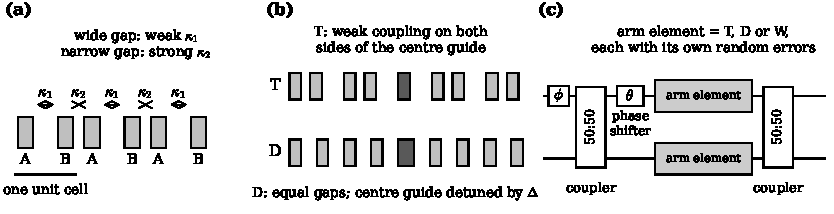
\includegraphics[width=0.88\textwidth]{fig1_schematic.pdf}
\caption{(a) Cross section of an SSH array: identical guides, alternating wide and narrow gaps. (b) The two arrays compared: T has a wide gap on both sides of its centre guide (dark); D has equal gaps and a centre guide with a shifted propagation constant. (c) One MZI of the simulated mesh, with an ``arm element'' in each arm.}
\label{fig:sch}
\end{figure*}
\shead{Bloch bands}In the SSH array the gaps alternate, so the couplings alternate too: $\ka,\kc,\ka,\dots$ (Fig.~\ref{fig:sch}a). Each unit cell has two guides, A and B, with amplitudes $a_n$, $b_n$. Equation~\eqref{eq:cmt} becomes
\begin{equation}
\frac{\dd a_n}{\dd z}=i(\ka b_n+\kc b_{n-1}),\quad \frac{\dd b_n}{\dd z}=i(\ka a_n+\kc a_{n+1}).
\label{eq:ssh}
\end{equation}
An A guide is linked only to B guides, and a B guide only to A guides. A long array looks the same after a shift of one cell. So, by Bloch's theorem, its modes change only by a phase from cell to cell: $a_n=a\,e^{ikn}$, $b_n=b\,e^{ikn}$, with $k\in(-\pi,\pi]$. Putting this into \eqref{eq:ssh} gives a $2\times2$ matrix $H(k)=\big(\begin{smallmatrix}0&h(k)\\h^*(k)&0\end{smallmatrix}\big)$ with $h(k)=\ka+\kc e^{-ik}$. Its two eigenvalues give the bands,
\begin{equation}
b_\pm(k)=\pm|h(k)|=\pm\sqrt{\ka^2+\kc^2+2\ka\kc\cos k}\, ,
\label{eq:bands}
\end{equation}
since $\det[H(k)-b]=b^2-|h|^2$ and $|h|^2=(\ka+\kc\cos k)^2+\kc^2\sin^2k$. The largest $|b|$ is $\ka+\kc$ and the smallest is $|\ka-\kc|$. So there is a \emph{band gap} of width $2|\ka-\kc|$ around $b=0$ where no bulk mode can live. It closes only when $\ka=\kc$. Swapping $\ka$ and $\kc$ does not change \eqref{eq:bands}, so the bands alone cannot tell the two patterns apart. A direct check on a ring of 48 guides matches these bands to $10^{-15}$ (Fig.~\ref{fig:theory}a).

\shead{Chiral symmetry pins a single mode at $b=0$}Define $\Gamma=\mathrm{diag}(+1,-1,+1,\dots)$, which is $+1$ on A guides and $-1$ on B guides. Then $(\Gamma H\Gamma)_{mn}=\gamma_mH_{mn}\gamma_n$ with $\gamma=\pm1$. A link from A to B has $\gamma_m\gamma_n=-1$, so it changes sign. A diagonal entry, or a link between two A guides, does not change sign. So, if and only if $H$ has no diagonal entries and only links A guides to B guides,
\begin{equation}
\Gamma H\Gamma=-H .
\label{eq:chiral}
\end{equation}
This is called chiral symmetry. It holds for \emph{any} coupling values, even random ones, and it gives two results. (i) If $H\psi=b\psi$ then $H(\Gamma\psi)=-\Gamma H\psi=-b(\Gamma\psi)$, so modes come in pairs $\pm b$. (ii) A mode at $b=0$ is its own partner. If it is the only one, it cannot move away from zero, because moving would need a twin at $-b$. Think of $b=0$ as a mirror: a single mode sitting on the mirror cannot leave it. \emph{Gap errors change only couplings and keep the symmetry. Width errors change diagonal entries and break it.}

\begin{figure}[!tb]\centering
\includegraphics[width=\columnwidth]{a.png}
\caption{A real SSH lattice: silicon nanowires with alternating gaps (electron microscope). The shaded guides sit at wide gap interfaces, which hold the edge mode of Eq.~(7). Reproduced from Wang \emph{et al.} (2019), Fig.~1.}\label{fig:ph-ssh}
\end{figure}
\shead{Winding number and the edge mode}The bands cannot tell the two patterns apart, but a whole number called the winding number can. Fig.~\ref{fig:ph-ssh} shows a real SSH array of this kind in silicon. Writing $h=d_x-id_y$ gives $d_x=\ka+\kc\cos k$ and $d_y=\kc\sin k$. As $k$ goes once round, the point $(d_x,d_y)$ draws a circle of radius $\kc$ around $(\ka,0)$ (Fig.~\ref{fig:theory}c). The winding number $W=\frac{1}{2\pi}\oint\dd\varphi$, with $\varphi=\arg(d_x+id_y)$, counts how many times this circle goes round the origin: $W=1$ if $\ka<\kc$ and $W=0$ if $\ka>\kc$. This count can only change if the circle passes through the origin, which means $|h|=0$ and the gap closes.

\begin{figure*}[!t]\centering
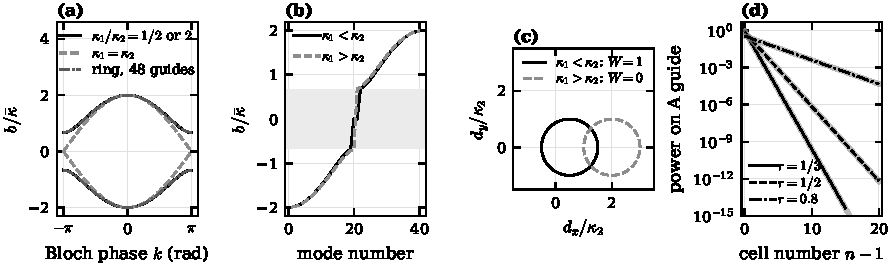
\includegraphics[width=0.88\textwidth]{fig2_theory.pdf}
\caption{Checks of the SSH theory. (a) Bands of Eq.~\eqref{eq:bands} in units of the mean coupling $\kb$; the dash-dot line shows the eigenvalues of a ring of 48 guides found by direct diagonalisation. (b) All eigenvalues of an open chain of 40 guides: two modes appear inside the gap (shaded) only when the end guide sits on the weak link. (c) The loop $(d_x,d_y)$ either encloses the origin or not. (d) Power of the zero mode on successive A guides of a chain of 41 guides (black lines) and Eq.~\eqref{eq:edge} (thick grey lines); the $r=1/3$ data stop at numerical roundoff.}
\label{fig:theory}
\end{figure*}
\mhead{Edge mode}Consider a chain that starts on an A guide and goes on without end. Look for a mode with $b=0$ and no light on the B guides ($b_n=0$). The first of Eqs.~\eqref{eq:ssh} is then true, and the second gives $0=\ka a_n+\kc a_{n+1}$, so
\begin{equation}
a_n=a_1(-r)^{n-1},\quad r=\frac{\ka}{\kc},\quad
\xi=\frac{1}{\ln(\kc/\ka)},
\label{eq:edge}
\end{equation}
where $\xi$ (in cells) is the length over which the amplitude falls by $1/e$. The mode has finite power only if $r<1$. This means the end guide must sit on the \emph{weak} link, which is the $W=1$ case. So there is one edge mode for each unit of $W$ (Ozawa \emph{et al.}). Normalising gives $|a_1|^2=1-r^2$. For $r=1/3$, $\xi=0.91$ cells and $89\%$ of the power is in the first guide. The computed mode follows $r^{2(n-1)}$ (Fig.~\ref{fig:theory}d).

%======================================================================
\section{A Fair Comparison and the Error Models}
\shead{Array T (topological) and array D (ordinary defect)}To see if topology really helps, the topological mode is compared with an ordinary mode of the same size. \textbf{Array T} has a centre guide with the weak coupling $\ka$ on both sides, and then the couplings alternate outward (Fig.~\ref{fig:sch}b). By Eq.~\eqref{eq:edge}, its mode is $\psi_{2j}=\psi_0(-r)^{|j|}$, $\psi_{2j+1}=0$, with $b_T=0$ exactly. \textbf{Array D} has all couplings equal to $\kb$, and its centre guide has its propagation constant raised by $\Delta$. Trying $\psi_n=q^{|n|}$, the equation away from the centre, $b\,\psi_n=\kb(\psi_{n-1}+\psi_{n+1})$, gives $b=\kb(q+1/q)$, and the centre gives $b=\Delta+2\kb q$. Equating the two,
\begin{equation}
\kb\Big(\frac1q-q\Big)=\Delta,\qquad b_D=\sqrt{\Delta^2+4\kb^2}\, .
\label{eq:D}
\end{equation}
Nothing pins this mode. The two modes are matched by their \emph{inverse participation ratio}, which measures how tightly a mode is packed (1 means all the light is in one guide):
\dmath{{\rm IPR}=\sum_n|\psi_n|^4=\frac{(1+q^4)(1-q^2)}{(1+q^2)^3}.}
T has the same formula with $q\to r$, so equal IPR means $q=r$. This work uses $r=1/3$, close to the value measured by Blanco Redondo \emph{et al.}, and gives everything in units of $\kc$ (so $\ka=1/3$, $\kb=2/3$). Then $\Delta=\frac{16}{9}\kc$, $b_D=\frac{20}{9}\kc$ and ${\rm IPR}=0.656$ for both (Fig.~\ref{fig:prop}a). Both modes also take the same share, $(1-r^2)/(1+r^2)=0.8$, of light put into the centre guide.

\shead{Error models and first order prediction}\emph{Gap errors} change each coupling as $\kappa\to\kappa\,e^{\sigma_\kappa g}$, where $g$ is a random Gaussian number and $\sigma_\kappa=\gamma\sigma_g$ (Eq.~\eqref{eq:gap}). They keep chiral symmetry. \emph{Width errors} shift each guide by $\delta\beta_n=\sigma_\beta g_n$, and they break it. A \emph{mixed} model lets one width error per guide cause both. For small errors, first order perturbation theory gives the shift $\delta b=\langle\psi|\delta H|\psi\rangle$:
\begin{equation}
\delta b\approx\sum_n\psi_n^2\,\delta\beta_n+2\sum_n\psi_n\psi_{n+1}\,\delta\kappa_n .
\label{eq:pt}
\end{equation}
For width errors both arrays get the same spread, because their IPR was matched:
\dmath{\sigma_\beta\Big(\sum_n\psi_n^4\Big)^{1/2}=\sigma_\beta\sqrt{\rm IPR}=0.81\,\sigma_\beta .}
For gap errors, T has $\psi_n\psi_{n+1}=0$ on every link, because every second guide is empty, so its shift is zero. In D, neighbouring guides both carry light. With $\psi_n^2=0.8\,q^{2|n|}$ and $\delta\kappa_n=\kb\sigma_\kappa g_n$, the variance is
\dmath{4\kb^2\sigma_\kappa^2\sum_n\psi_n^2\psi_{n+1}^2=4\kb^2\sigma_\kappa^2\cdot\frac{2(0.8)^2q^2}{1-q^4},}
so the spread of D is $0.51\,\sigma_\kappa\kc$.

%======================================================================
\section{Simulated Chips: Eigenvalue, Propagation and Phase}
\begin{figure*}[!t]\centering
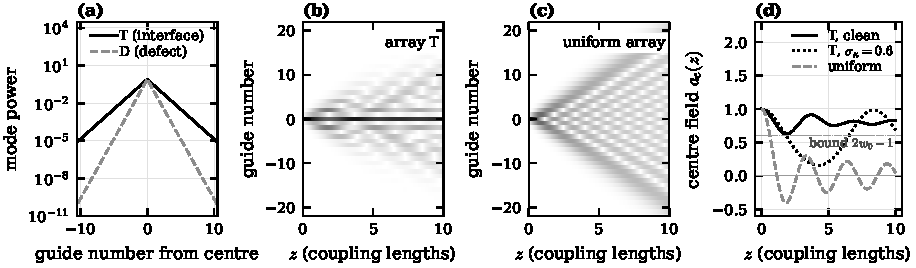
\includegraphics[width=0.88\textwidth]{fig3_propagation.pdf}
\caption{Design and propagation. (a) Power of the T and D modes with equal IPR; T is zero on every second guide. (b) Light launched into the centre guide of array T (81 guides): 80\% stays bound, the rest spreads. Grey level shows field amplitude. (c) The same launch in a uniform array gives discrete diffraction. (d) Field in the centre guide: always real in a chiral array; for clean T it stays above the bound $2w_0-1=0.6$, while the uniform array changes sign.}
\label{fig:prop}
\end{figure*}
\shead{Pinning of the eigenvalue}For each error strength, 2000 random chips of 41 guides were made, and the mode closest to the clean one was followed (Fig.~\ref{fig:mc}a,b). Under gap errors, T stays at $b=0$ to within $10^{-15}\kc$, which is just computer round off. D spreads as $0.508\,\sigma_\kappa$ (predicted 0.506). Under width errors, T and D spread \emph{equally}: $0.815$ and $0.805$ times $\sigma_\beta$ (predicted 0.810). So topology removes one kind of error completely and does nothing about the other. It also protects only the number $b$, not the shape of the mode: at $\sigma_\kappa=0.3$, the power of T's mode in the centre guide drops on average from 0.80 to 0.75.

\shead{Propagation and the phase}A fixed $b$ alone does not fix the phase of the light leaving the arm, because the input light excites more than one mode. Light put into the centre guide $c$ evolves as
\dmath{\bm a(z)=\sum_m\langle\psi_m|\bm a(0)\rangle e^{ib_mz}\psi_m ,}
so each mode turns its phase at its own rate (Fig.~\ref{fig:prop}b,c). Fig.~\ref{fig:ph-out} shows the same contrast measured in silicon. The field that comes back out of guide $c$ is
\begin{equation}
a_c(z)=\sum_m|\psi_m(c)|^2e^{ib_mz}=w_0+\sum_{b_m>0}2|\psi_m(c)|^2\cos b_mz ,
\label{eq:real}
\end{equation}
where the $\pm b$ pairs of Section~III were used and $w_0=|\psi_0(c)|^2$ is the weight of the zero mode. This says two things. First, \emph{$a_c(z)$ is real in any chiral array}, so its phase can only be 0 or $\pi$. This needs only the symmetry, not topology. Second, the cosine terms add up to at most $1-w_0$, so $a_c\ge2w_0-1$. If $w_0>1/2$, the field never changes sign and the phase stays at 0 for every length. For clean T, $w_0=0.8$ and $a_c\ge0.6$. The uniform array has no zero mode, and its field swings down to $-0.40$ (Fig.~\ref{fig:prop}d). Width errors make $a_c$ complex, and the phase error then grows with length as $\delta b\,L$.

\begin{figure}[!tb]\centering
\includegraphics[width=\columnwidth]{b.png}
\caption{Measured light leaving silicon arrays at five wavelengths (1546 to 1554 nm): short short defect (top), equal gaps (middle) and long long topological defect (bottom). Reproduced from Blanco Redondo \emph{et al.} (2016).}\label{fig:ph-out}
\end{figure}
\mhead{Loss}Uniform loss only makes the light weaker. Unequal loss gives $\Gamma H\Gamma=-H^\dagger$, so the zero mode keeps ${\rm Re}\,b=0$: it fades, but its phase stays pinned (Weimann \emph{et al.}).

\begin{figure*}[!t]\centering
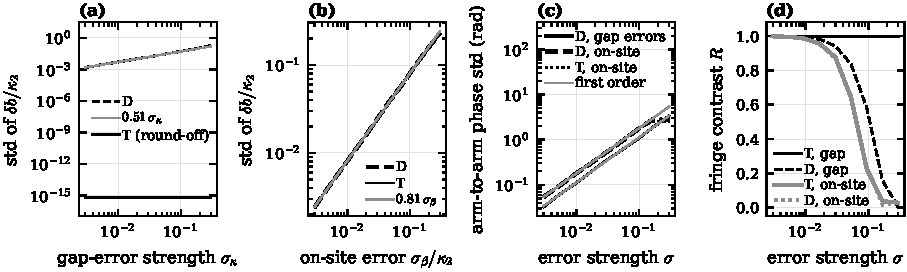
\includegraphics[width=0.88\textwidth]{fig4_montecarlo.pdf}
\caption{Monte Carlo results (2000 simulated chips per point; lines are the first order predictions of Section~IV). (a) Spread of the mode's propagation constant shift under gap errors: D follows $0.51\sigma_\kappa$, T stays at roundoff. (b) Under on site (width) errors T and D are equal. (c) Arm to arm phase error after 10 coupling lengths; T under gap errors is exactly zero and cannot be drawn on this scale. (d) Fringe contrast $R$ that an interferometer would keep.}
\label{fig:mc}
\end{figure*}
\shead{The phase an interferometer sees}An interferometer only sees the phase \emph{difference} $\Delta\varphi$ between its two arms, so any error shared by the whole chip cancels. Pairs of arms were simulated, each with its own errors and each $L=10$ coupling lengths long ($L=5\pi/\kc$). When $\Delta\varphi$ is random, the fringe $\cos(\theta+\Delta\varphi)$ is weakened on average by the factor $R=|\langle e^{i\Delta\varphi}\rangle|$, the fringe contrast that is left (Fig.~\ref{fig:mc}c,d). For gap errors, T has $\Delta\varphi=0$ exactly up to $\sigma_\kappa=0.17$, and $R=1.00$ at $\sigma_\kappa=0.095$, where D has already fallen to $R=0.58$. For width errors, T and D behave the same: 0.53~rad each at $\sigma_\beta=0.03\kc$. There is a cost: under gap errors the output \emph{power} of T varies four to five times more than that of D, because the pinned mode changes shape.

%======================================================================
\section{From One Arm to an MZI Mesh}
\shead{Coupler, MZI and mesh fidelity}A directional coupler is just an array of two guides, so $\dd\bm a/\dd z=i\kappa\sigma_x\bm a$ with $\sigma_x=\big(\begin{smallmatrix}0&1\\1&0\end{smallmatrix}\big)$. Because $\sigma_x^2=I$, a coupler of length $\ell$ is
\begin{equation}
B=\cos\kappa\ell\;I+i\sin\kappa\ell\;\sigma_x=\begin{pmatrix}\sqrt\eta&i\sqrt{1-\eta}\\ i\sqrt{1-\eta}&\sqrt\eta\end{pmatrix},\qquad\eta=\cos^2\kappa\ell ,
\label{eq:B}
\end{equation}
where $\eta$ is the share of power that stays in its own guide. A 50:50 split needs $\kappa\ell=\pi/4$. Since $\dd\eta=-\sin(2\kappa\ell)\,\kappa\ell\,(\delta\kappa/\kappa)$, a gap error there gives a splitting error $\sigma_\eta=\frac{\pi}{4}\sigma_\kappa$. A phase shifter is $P(\phi)={\rm diag}(e^{i\phi},1)$. An MZI is $B\,P(\theta)\,B\,P(\phi)$ (Fig.~\ref{fig:sch}c), and Fig.~\ref{fig:ph-mzi} shows real MZIs tuned by heaters. With $\eta=\frac12$,
\begin{equation}
B\,P(\theta)\,B=i\,e^{i\theta/2}\begin{pmatrix}\sin\frac\theta2&\cos\frac\theta2\\[1pt] \cos\frac\theta2&-\sin\frac\theta2\end{pmatrix},
\label{eq:mzi}
\end{equation}
so $\theta$ sets the split and $\phi$ sets the phase. With imperfect couplers some light is always left in the wrong port: 1\% for $\eta=0.45$ and 4\% for $\eta=0.40$ (Fig.~\ref{fig:circ}a; Miller).

\begin{figure}[!tb]\centering
\includegraphics[width=\columnwidth]{e.png}
\caption{Real tunable beam splitters: MZIs whose phase is set by a heater on one arm. Reproduced from Buzaverov \emph{et al.} (2023), Fig.~12(f).}\label{fig:ph-mzi}
\end{figure}
Many MZIs together form a mesh (Fig.~\ref{fig:ph-mesh}). A rectangular mesh (Clements \emph{et al.}) of size $N$ has $N(N-1)/2$ MZIs and $N^2$ phase shifters. To compare the real mesh $U$ with the ideal $U_0$, the fidelity
\dmath{F=\frac{|\Tr(U_0^\dagger U)|^2}{N\,\Tr(U^\dagger U)}}
is used. It equals 1 only if $U=U_0$, up to a common phase and a uniform loss. One phase error $\delta$ on one path multiplies the mesh by a matrix $W$ with $\Tr W=N-1+e^{i\delta}$, so
\dmath{|\Tr W|^2=(N-1)^2+1+2(N-1)\cos\delta\approx N^2-(N-1)\delta^2 ,}
and this one error costs $1-F=(N-1)\delta^2/N^2$. Independent errors add. For $N^2$ shifters, and in the same way for $N(N-1)$ couplers, this gives
\begin{equation}
1-F\approx(N-1)\,\sigma_\phi^2,\qquad 1-F\approx2(N-1)\,\sigma_\eta^2 .
\label{eq:mesh}
\end{equation}
Simulated meshes with $N=4,6,8$ agree with \eqref{eq:mesh} within 1\% (Fig.~\ref{fig:circ}b).

\begin{table*}[!t]
\centering
\caption{Simulated circuit results for arm elements T, D and W (arms 10 coupling lengths long). Left: infidelity $1-F$ of an $N=6$ mesh at error strength $\sigma=0.01$. Right: mean HOM visibility when an MZI with these arms is used as the 50:50 splitter.}
\label{tab:res}
\begin{tabular}{@{}lccc@{\hspace{2.2em}}lccc@{}}\toprule
Mesh infidelity $1-F$ & T & D & W & Mean HOM visibility $V$ & T & D & W\\\midrule
gap errors, arms only & $2.5\times10^{-4}$ & $0.027$ & $0$ & gap errors, $\sigma_\kappa=0.01$ & 0.9998 & 0.975 & 1\\
gap errors, arms and couplers & $8.7\times10^{-4}$ & $0.027$ & $6.2\times10^{-4}$ & gap errors, $\sigma_\kappa=0.03$ & 0.998 & 0.835 & 1\\
width (on site) errors & $0.060$ & $0.064$ & $0.097$ & width errors, $\sigma_\beta=0.01\kc$ & 0.947 & 0.942 & 0.917\\
mixed, $\sigma_\beta=\sigma_\kappa$, with couplers & $0.062$ & $0.144$ & $0.098$ & width errors, $\sigma_\beta=0.03\kc$ & 0.701 & 0.692 & 0.618\\\bottomrule
\end{tabular}
\end{table*}
\begin{figure*}[!t]\centering
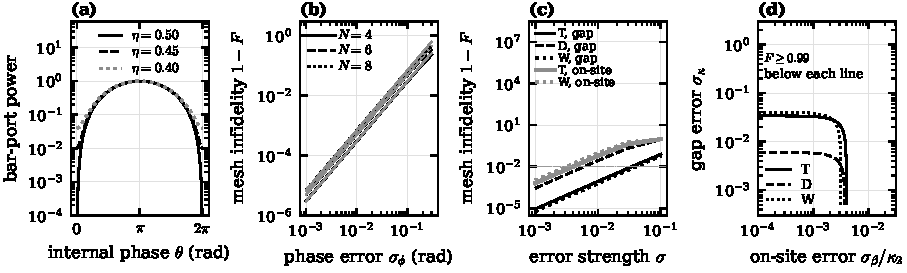
\includegraphics[width=0.88\textwidth]{fig5_circuits.pdf}
\caption{Circuit level results. (a) Power left in the wrong (bar) port of one MZI against $\theta$: with ideal couplers it reaches zero, with $\eta=0.45$ and $0.40$ it stops at 1\% and 4\%. (b) Infidelity of rectangular meshes with random phase errors; lines are Eq.~\eqref{eq:mesh}. (c) Infidelity of an $N=6$ mesh whose arms are T, D or W elements; gap error curves include coupler errors; the horizontal line marks $F=0.99$. (d) Boundary $F=0.99$ from Eq.~\eqref{eq:crit} for independent on site and gap errors.}
\label{fig:circ}
\end{figure*}
\begin{figure}[!tb]\centering
\includegraphics[width=0.9\columnwidth]{c.png}
\caption{A programmable processor built from a mesh of MZIs (outlined), used as the linear layer of an optical neural network. Reproduced from Shen \emph{et al.} (2017), Fig.~2.}\label{fig:ph-mesh}
\end{figure}
\shead{Arrays as interferometer arms}Next, each MZI arm in the mesh gets one arm element: T, D, or a plain single waveguide W of the same length, used for comparison (Fig.~\ref{fig:sch}c). A small amplitude error costs as much fidelity as a phase error of the same size. With $N(N-1)$ arms this gives
\begin{equation}
1-F\approx\frac{(N-1)^2}{N}\Big[(c_\beta\,\sigma_\beta L)^2+(c_\kappa\,\sigma_\kappa)^2\Big]+2(N-1)\Big(\frac{\pi}{4}\sigma_\kappa\Big)^2 .
\label{eq:crit}
\end{equation}
The numbers $c_\beta$ and $c_\kappa$ were found from 4000 simulated arms with $L=15.7/\kc$. For width errors, $c_\beta\approx0.8$ for the arrays ($=\sqrt{\rm IPR}$) and 1 for W. For gap errors, $c_\kappa=0.77$ for T (amplitude only), $8.1$ for D (phase) and 0 for W. Full mesh simulations ($N=6$, 400 meshes per point; Table~\ref{tab:res}, Fig.~\ref{fig:circ}c) agree with \eqref{eq:crit} within a few per cent when $1-F<0.1$.

In short: (1) Against gap errors, T is about 100 times better than D, and the error left in T is in amplitude, not phase. (2) A plain waveguide does just as well, because it has no couplings for a gap error to act on. (3) Against width errors, T and D are equal. (4) The fidelity does not show insertion loss: a clean T arm sends only 0.694 of its power back to the centre guide, so six arms in a row pass only $0.694^6\approx0.11$. Fig.~\ref{fig:circ}d shows where $F\ge0.99$. Width errors set the limit: every element needs $\sigma_\beta\lesssim0.004\,\kc$. For gap errors, couplers included, the limit is $\sigma_\kappa\approx0.035$ for T, 0.04 for W and 0.006 for D.

%======================================================================
\section{Quantum Extension: HOM Interference}
Send one photon into each input of a beam splitter. With the coupler \eqref{eq:B}, the photon operators change as
\dmath{a^\dagger\to\sqrt\eta\,c^\dagger+i\sqrt{1-\eta}\,d^\dagger,\qquad b^\dagger\to i\sqrt{1-\eta}\,c^\dagger+\sqrt\eta\,d^\dagger .}
The case with one photon in each output is called a ``coincidence'', and its amplitude is $\eta+i^2(1-\eta)=2\eta-1$. The two ways to get a coincidence cancel, so the coincidence probability $P_c=(2\eta-1)^2$ is zero at 50:50. Identical photons always leave together (Hong, Ou and Mandel). If the photons are not identical, with internal states $\rho_1$ and $\rho_2$, only the part they share can interfere:
\dmath{P_c=R^2+T^2-2RT\,\Tr(\rho_1\rho_2),\qquad T=\eta,\ R=1-\eta .}
The visibility $V$ is the depth of the dip:
\begin{equation}
V=\frac{2RT}{R^2+T^2}\,\Tr(\rho_1\rho_2) .
\label{eq:hom}
\end{equation}
\begin{figure*}[!t]\centering
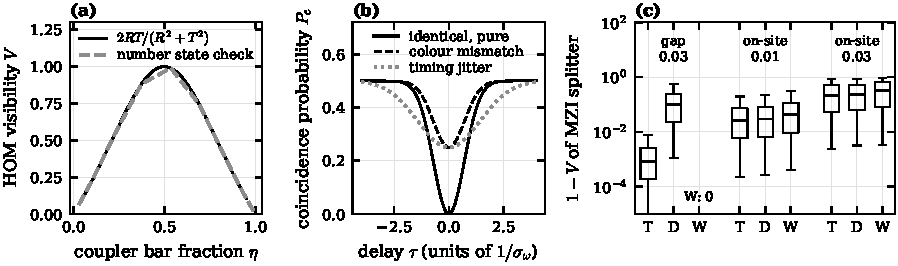
\includegraphics[width=0.88\textwidth]{fig6_hom.pdf}
\caption{HOM interference. (a) Visibility against the coupler splitting ratio, Eq.~\eqref{eq:hom}; the dashed line is an independent number state calculation. (b) Coincidence dips for identical pure photons, for a colour mismatch and for timing jitter, the last two both set to $V=0.5$: jitter widens the dip. (c) Spread of $1-V$ over 4000 MZI splitters whose arms are T, D or W elements (box: middle half; bars: 5\% to 95\%). For gap errors W has $V=1$ exactly.}
\label{fig:hom}
\end{figure*}
A separate number state calculation agrees to $10^{-16}$ (Fig.~\ref{fig:hom}a). Two different effects can lower $V$. \emph{Distinguishability} means the two photons are in pure but different states, for example of different colour. \emph{Decoherence} means each photon is in a mixed state, for example because of random timing jitter. Both lower $V$ in the same way, so $V$ alone cannot tell them apart. The shape of the dip can: a colour mismatch that gives $V=0.5$ keeps the dip width at 1.64 (in units of $1/\sigma_\omega$), while jitter that gives the same $V$ doubles it to 3.32 (Fig.~\ref{fig:hom}b).

\begin{figure}[!tb]\centering
\includegraphics[width=0.9\columnwidth]{f.png}
\caption{On chip interference of heralded photons from two separate silicon sources (inset): the fourfold detection count against the MZI phase $\theta_1$ falls almost to zero at $\pi/2$. Reproduced from Paesani \emph{et al.} (2020).}\label{fig:ph-hom}
\end{figure}
\mhead{Role of the arm phase}For a coupler with $\eta=\frac12+\delta$, Eq.~\eqref{eq:hom} gives $V\approx1-8\delta^2$, and with $\delta=\frac{\pi}{4}\sigma_\kappa$ this is $V\approx1-\frac{\pi^2}{2}\sigma_\kappa^2$. The arm phase matters only when the splitter is itself an MZI set to $\theta=\pi/2$, as in the experiment of Fig.~\ref{fig:ph-hom}. With arms made of T, D or W (Table~\ref{tab:res}, Fig.~\ref{fig:hom}c), the result follows the classical circuit. T keeps the interference against gap errors, much better than D but no better than a plain guide. Against width errors T gives no help: the worst 5\% of MZIs fall to $V\approx0.16$ at $\sigma_\beta=0.03\kc$.

%======================================================================
\section{Discussion and Conclusion}
\mhead{Summary}Topological protection protects the interferometric phase \emph{only partly, and only for one kind of error}. Gap errors (and unequal loss) keep chiral symmetry. They leave the phase of the topological mode exactly unchanged, from the eigenvalue up to the mesh and the HOM visibility. But the error does not disappear; it moves into the amplitude. Width errors break the symmetry, are not reduced at all, and set the tolerance. Even for gap errors, a plain single waveguide is equally safe and has no insertion loss.

\mhead{Design criterion}A topological array is worth using as an interferometer arm only when (i) the guides are packed so closely that they couple anyway, (ii) gap errors are much larger than width errors, that is $c_\kappa\sigma_\kappa$ is large compared with $\sigma_\beta L$, and (iii) its insertion loss can be accepted. Otherwise a plain waveguide is the better arm.

\mhead{Limitations}Only nearest neighbour couplings are kept, although longer range coupling also breaks chiral symmetry. Tolerances are in units of $\kc$, not nanometres, because the real coupling and $\sigma_\beta/\sigma_\kappa$ are not known. Only $N=6$ meshes with independent errors were simulated, and the HOM model covers two photons in one $2\times2$ device.

\mhead{Code and data}Simulation code, data and figure scripts: \url{https://github.com/Kishore-Kotapati/TOP-Q}.

\section*{References}
{\footnotesize
\begin{enumerate}
\renewcommand{\labelenumi}{\arabic{enumi}.}
\setlength{\itemsep}{0pt}\setlength{\parskip}{0pt}\setlength{\leftmargin}{1.6em}
\item M. Reck, A. Zeilinger, H. J. Bernstein, and P. Bertani, ``Experimental realization of any discrete unitary operator,'' Phys. Rev. Lett. \textbf{73}, 58--61 (1994).
\item Y. Shen \emph{et al.}, ``Deep learning with coherent nanophotonic circuits,'' Nat. Photonics \textbf{11}, 441--446 (2017).
\item M. Y.-S. Fang, S. Manipatruni, C. Wierzynski, A. Khosrowshahi, and M. R. DeWeese, ``Design of optical neural networks with component imprecisions,'' Opt. Express \textbf{27}, 14009--14029 (2019).
\item T. Ozawa \emph{et al.}, ``Topological photonics,'' Rev. Mod. Phys. \textbf{91}, 015006 (2019).
\item W. P. Su, J. R. Schrieffer, and A. J. Heeger, ``Solitons in polyacetylene,'' Phys. Rev. Lett. \textbf{42}, 1698--1701 (1979).
\item A. Blanco-Redondo \emph{et al.}, ``Topological optical waveguiding in silicon and the transition between topological and trivial defect states,'' Phys. Rev. Lett. \textbf{116}, 163901 (2016).
\item C. K. Hong, Z. Y. Ou, and L. Mandel, ``Measurement of subpicosecond time intervals between two photons by interference,'' Phys. Rev. Lett. \textbf{59}, 2044--2046 (1987).
\item A. Blanco-Redondo, B. Bell, D. Oren, B. J. Eggleton, and M. Segev, ``Topological protection of biphoton states,'' Science \textbf{362}, 568--571 (2018).
\item W. R. Clements, P. C. Humphreys, B. J. Metcalf, W. S. Kolthammer, and I. A. Walmsley, ``Optimal design for universal multiport interferometers,'' Optica \textbf{3}, 1460--1465 (2016).
\item A. Yariv, ``Coupled-mode theory for guided-wave optics,'' IEEE J. Quantum Electron. \textbf{9}, 919--933 (1973).
\item S. Weimann \emph{et al.}, ``Topologically protected bound states in photonic parity--time-symmetric crystals,'' Nat. Mater. \textbf{16}, 433--438 (2017).
\item D. A. B. Miller, ``Perfect optics with imperfect components,'' Optica \textbf{2}, 747--750 (2015).
\item M. Wang, C. Doyle, B. Bell, M. J. Collins, E. Magi, B. J. Eggleton, M. Segev, and A. Blanco-Redondo, ``Topologically protected entangled photonic states,'' Nanophotonics \textbf{8}, 1327--1335 (2019).
\item K. A. Buzaverov \emph{et al.}, ``Low-loss silicon nitride photonic ICs for near-infrared wavelength bandwidth,'' Opt. Express \textbf{31}, 16227--16242 (2023).
\item S. Paesani, M. Borghi, S. Signorini, A. Ma\"inos, L. Pavesi, and A. Laing, ``Near-ideal spontaneous photon sources in silicon quantum photonics,'' Nat. Commun. \textbf{11}, 2505 (2020).
\end{enumerate}}

\section*{Acknowledgement}\small
I want to extend my hearty gratitude to Prof. Sivarama Krishnan for providing me with this opportunity to craft this term paper. I would also like to thank the Department of Physics for nurturing me as a student.



\end{document}
